\documentclass{scrartcl}

\usepackage[hw]{darkwhite}

\title{18.676 Stochastic Calculus}
\subtitle{Problem Set 1}



\begin{document}
% Exercise 1.15 Let .Xt/t2Œ0;1 be a centered Gaussian process. We assume that the
% mapping .t;!/ 7! Xt.!/ from Œ0; 1  ˝ into R is measurable. We denote the
% covariance function of X by K.
% 1. Show that the mapping t 7! Xt from Œ0; 1 into L2.˝/ is continuous if and only if
% K is continuous on Œ0; 12: In what follows, we assume that this condition holds.
% 2. Let h W Œ0; 1 ! R be a measurable function such that R 1
% 0 jh.t/j
% pK.t; t/ dt < 1:
% Show that, for a.e. !, the integral R 1
% 0 h.t/Xt.!/dt is absolutely convergent. We set
% Z D R 1
% 0 h.t/Xtdt.
% 3. We now make the stronger assumption R 1
% 0 jh.t/jdt < 1. Show that Z is the L2-
% limit of the variables Zn D Pn
% iD1 X i
% n
% R i
% n
% i1
% n
% h.t/dt when n ! 1 and infer that Z is
% a Gaussian random variable.
% Exercises 15
% 4. We assume that K is twice continuously differentiable. Show that, for every t 2
% Œ0; 1, the limit
% XPt WD lim
% s!t
% Xs  Xt
% s  t
% exists in L2.˝/: Verify that .XPt/t2Œ0;1 is a centered Gaussian process and compute
% its covariance function.
\section{Centered Gaussian Processes}

\begin{prob*}
    Let $(X_t)_{t \in [0,1]}$ be a centered Gaussian process. We assume that the mapping $(t,\omega) \mapsto X_t(\omega)$ from $[0,1] \times \Omega$ into $\RR$ is measurable. We denote the covariance function of $X$ by $K$.
\end{prob*}

\begin{prob}
    Show that the mapping $t \mapsto X_t$ from $[0,1]$ into $L^2(\Omega)$ is continuous if and only if $K$ is continuous on $[0,1]^2$. In what follows, we assume that this condition holds.
\end{prob}

We first assume that $K$ is continuous on $[0,1]^2$. Fix $t\in [0,1]$ and $\eps > 0$. By continuity at $(t,t)\in [0,1]^2$, we find that there exists a $\delta > 0$ such that for all $u, v \in [t - \delta', t + \delta']$, we have $\abs{K(u,v) - K(t,t)} < \eps^2 / 3$. Then, for all $s \in [0,1]$ with $\abs{t-s} < \delta$,
\[
    \EE[(X_t - X_s)^2] = K(t,t) - 2K(t,s) + K(s,s) < 0 + 2\eps^2/3 + \eps^2/3 = \eps^2.
\]
thus
\[
    \norm{X_t - X_s}_2 < \eps.
\]

Conversely, assume that $t \mapsto X_t$ is continuous. Then, $t\mapsto X_t \mapsto \norm{X_t}^2$ is continuous. $[0,1]$ is compact, thus $\norm{X_t}^2$ attains some maximum value $M$. Fix $(t_1,t_2) \in [0,1]^2$ and $\eps > 0$. By continuity at $t_1$, we find a $\delta_1 > 0$ such that for all $s \in [t_1 - \delta_1, t_1 + \delta_1]$, we have $\norm{X_{t_1} - X_s}_2 < \frac{\eps}{2M}$. Define $\delta_2$ similarly. Then, for all $s_1 \in [t_1 - \delta_1, t_1 + \delta_1]$ and $s_2 \in [t_2 - \delta_2, t_2 + \delta_2]$,
\begin{align*}
    \abs{K(s_1,s_2) - K(t_1,t_2)} &= \abs{\EE[X_{s_1} X_{s_2} - X_{t_1} X_{t_2}]}\\
    &\leq \abs{\EE[X_{s_1}(X_{s_2} - X_{t_2})]} + \abs{\EE[(X_{s_1} - X_{t_1})X_{t_2}]} \tag{Triangle Inequality}\\
    &\leq \norm{X_{s_1}}\norm{X_{s_2} - X_{t_2}} + \norm{X_{s_1} - X_{t_1}}\norm{X_{t_2}} \tag{Cauchy-Schwarz}\\
    &< M \frac{\eps}{2M} + \frac{\eps}{2M}M = \eps.
\end{align*}
as desired.

\begin{prob}
    Let $h \colon [0,1] \to \RR$ be a measurable function such that $\int_0^1 \abs{h(t)} \sqrt{K(t,t)} \, dt < \infty$. Show that, for a.e. $\omega$, the integral $\int_0^1 h(t)X_t(\omega) \, dt$ is absolutely convergent. We set $Z = \int_0^1 h(t)X_t \, dt$.
\end{prob}

\idea{
    [Key Ideas]
    A continuous function on a compact domain is uniformly continuous.

    We can take the measurable function $[0,1]\times \Omega \to \RR$ seriously.
}

It is well-known (and otherwise quickly computed) that
\[
    \int_\Omega \abs{X_t(\omega)} \, d\PP = \sqrt{\frac{2}{\pi}} \sqrt{K(t,t)}.  
\]
The constant term doesn't matter.

We simply compute
\begin{align*}
    \int_\Omega \int_0^1 \abs{h(t)X_t(\omega)} \, dt \, d\PP &= \int_0^1 \int_\Omega \abs{h(t)X_t(\omega)} \, d\PP \, dt \tag{Fubini's Theorem}\\
    &= \int_0^1 \abs{h(t)} \int_\Omega \abs{X_t(\omega)} \, d\PP \, dt\\
    &= \int_0^1 \abs{h(t)} \sqrt{\frac{2}{\pi}}\sqrt{K(t,t)} \, dt < \infty.
\end{align*}
Thus, for a.e. $\omega$, the integral $\int_0^1 h(t)X_t(\omega) \, dt$ is absolutely convergent.



\begin{prob}
    We now make the stronger assumption $\int_0^1 \abs{h(t)} \, dt < \infty$. Show that $Z$ is the $L^2$-limit of the variables
    \[
        Z_n = \sum_{i=1}^n X_{i/n} \int_{(i-1)/n}^{i/n} h(t) \, dt
    \]
    when $n \to \infty$ and infer that $Z$ is a Gaussian random variable.
\end{prob}

Let $M = \int_0^1 \abs{h(t)} \, dt$. Let's go ahead and compute the difference:
\begin{align*}
    Z_n - Z &= \sum_{i=1}^n X_{i/n} \int_{(i-1)/n}^{i/n} h(t) \, dt - \int_0^1 h(t)X_t \, dt\\
    &= \sum_{i=1}^n X_{i/n} \int_{(i-1)/n}^{i/n} h(t) \, dt - \sum_{i=1}^n \int_{(i-1)/n}^{i/n} h(t)X_t \, dt\\
    &= \sum_{i=1}^n \int_{(i-1)/n}^{i/n} h(t)(X_{i/n} - X_t) \, dt
\end{align*}
We now bound the norm of the whole thing, using triangle inequality.
\begin{align*}
    \norm{Z_n - Z}_2 &\leq \sum_{i=1}^n \int_{(i-1)/n}^{i/n} h(t)\norm{(X_{i/n} - X_t)}_2 \, dt
\end{align*}

By uniform continuity of $t \mapsto X_t$, for all $\eps > 0$, there exists a $\delta > 0$ such that for all $s \in [t - \delta, t + \delta]$, we have $\norm{X_t - X_s}_2 < \eps / M$. Then pick some $n > \frac{1}{\delta}$. We have
\begin{align*}
    &\leq \sum_{i=1}^n \int_{(i-1)/n}^{i/n} h(t)\eps / M \, dt\\
    &= \eps / M \int_0^1 \abs{h(t)} \, dt\\
    &= \eps.
\end{align*}
Thus, $Z_n \to Z$ in $L^2$. The limit of a $L^2$-convergent sequence of Gaussian random variables is a Gaussian random variable.

\begin{prob}
    We assume that $K$ is twice continuously differentiable. Show that, for every $t \in [0,1]$, the limit $\dot{X}_t = \lim_{s \to t} \frac{X_s - X_t}{s-t}$ exists in $L^2(\Omega)$. Verify that $(\dot{X}_t)_{t \in [0,1]}$ is a centered Gaussian process and compute its covariance function.
\end{prob}
Fix $t\in [0,1]$. For the first part, the existence of continuous second derivatives implies that $\exists \pa_{xy}K\forall \eps > 0 \exists \delta_\eps > 0$ such that $\forall \abs{\alpha},\abs{\beta} < \delta_\eps$,
\[
    \abs{\frac{K(t + \alpha, t + \beta) - K(t + \alpha, t) - K(t, t + \beta) + K(t,t)}{\alpha\beta} - \pa_{xy} K(t,t)} < \eps.
\]

Fix $t\in [0,1]$. We will show that $\dot{X}_t$ exists by showing that the sequence $Y_\alpha = \frac{X_{t + \alpha} - X_t}{\alpha}$ is Cauchy in $L^2$.
\idea{
    [Cauchy Criterion]
    For any $\eps > 0$, I will exhibit a $\abs{\delta} > 0$ such that for all $\abs{\delta} > \abs{\eta} > 0$, $\norm{Y_\delta - Y_\eta}_2 < \eps$.
}

Pick any $\eps$. Now, we will pick $\abs{\delta} = \delta_{\eps / 4}$ (where $\delta$ is defined as above). For any $\abs{\eta} < \abs{\delta}$, we have
\begin{align*}
    \norm{\frac{X_{t + \delta} - X_t}{\delta} - \frac{X_{t + \eta} - X_t}{\eta}}_2^2 &= \EE\left[\left(\frac{X_{t + \delta} - X_t}{\delta} - \frac{X_{t + \eta} - X_t}{\eta}\right)^2\right]\\
    &= \left\vert\frac{K(t + \delta, t + \delta) - 2K(t + \delta, t) + K(t,t)}{\delta^2}\right.\\
    &+ \frac{K(t + \eta, t + \eta) - 2K(t + \eta, t) + K(t,t)}{\eta^2}\\
    &\left.- 2\frac{K(t + \delta, t + \eta) - K(t + \delta, t) - K(t , t+ \eta) + K(t,t)}{\delta\eta}\right\vert\\
    & < \eps
\end{align*}
as desired.

% We know that the limit of a sequence of Gaussian RVs which converge in $L^2$ is another Gaussian RV, so each $\dot X_t$ is a centered Gaussian RV.
We need to show that $\dot{X}_t$ is a centered Gaussian \emph{process} i.e. any finite linear combination of $\dot{X}_t$'s is a centered Gaussian RV.
% This is basically clear though.
Let's investigate $\sum_i \alpha_i \dot{X}_i$ for some finite set of indices $i\in I\subset [0,1]$. By (finite) linearity of limits, this is equal to the $L^2$-limit of $\sum_i \alpha_i Y_{i, \delta}$ as $\delta \to 0$... but this is just a $L^2$-limit of a bunch of centered Gaussian RVs, so it's not too deep.  Let's compute the variance of this process in the case where $I = \{t,s\}$:
\begin{align*}
    \EE\left[ \left(\alpha_t Y_{t,\delta} + \alpha_s Y_{s,\delta}\right)^2\right] &= \EE\left[\alpha_t^2 Y_{t,\delta}^2 + 2\alpha_t\alpha_s Y_{t,\delta}Y_{s,\delta} + \alpha_s^2 Y_{s,\delta}^2\right]\\
    &= \alpha_t^2 \left( \frac{K(t + \delta, t + \delta) - 2K(t + \delta, t) + K(t,t)}{\delta^2}\right)\\
    &+ 2\alpha_t\alpha_s \left( \frac{K(t + \delta, s + \delta) - K(t + \delta, s) - K(t , s+ \delta) + K(t,s)}{\delta^2}\right)\\
    &+ \alpha_s^2 \left( \frac{K(s + \delta, s + \delta) - 2K(s + \delta, s) + K(s,s)}{\delta^2}\right)
\end{align*}
thus in the limit $\alpha_t X_t + \alpha_s X_s$ (from that same result on convergence of Gaussian RVs) is a centered Gaussian RV with variance
\[
    \alpha_t^2 \pa_{xy} K(t,t) + 2\alpha_t\alpha_s \pa_{xy} K(t,s) + \alpha_s^2 \pa_{xy} K(s,s).    
\]
This immediately shows that the covariance function of $\dot{X}$ is $\pa_{xy} K$ (by e.g. taking the results for $(\alpha_t, \alpha_s) = (1,0), (0,1), (1,1)$ and subtracting).

% By Taylor's theorem, we have a rather complicated but ultimately self-explanatory expansion and bound for $K$. Fix $(t,s)$. There exist functions $h_{xx}, h_{xy}, h_{yy}$ such that
% \begin{align*}
%     K(t + \alpha, t + \beta) &= K(t,s) + \alpha \pa_x K + \beta \pa_y K + \alpha^2 \frac{\pa_x^2 K}{2} + \alpha\beta \pa_{xy} K + \beta^2 \frac{\pa^2 K}{2}\\
%     &+ \alpha^2 h_{xx}(\alpha,\beta) + \alpha\beta h_{xy}(\alpha,\beta) + \beta^2 h_{yy}(\alpha,\beta)
% \end{align*}
% and in the limit as $\abs{\alpha} + \abs{\beta} \to 0$, all of $h_{xx}, h_{xy}, h_{yy}$ vanish.
% \idea{
%     However, as was rudely made apparent while solving this question, these conditions are not if and only if; the existence of continuous second
%     derivatives is strictly stronger than these statements; there are additional conditions on the $h_{ij}$.
% }

% By symmetry, let us call $A = \pa_x K = \pa_y K$, $B = \pa_{xx} K = \pa_{yy} K$, $C = \pa_{xy} K$, $h = h_{xx} = h_{yy}$, $.
% Then, for any $\eps, \delta$,


% Great. We expand the first term first (we drop linear terms which clearly vanish):
% \begin{align*}
%     \frac{K(t + \delta, t + \delta) - 2K(t + \delta, t) + K(t,t)}{\delta^2}
%     &= \pa_{xy} K(t,t) + h_{xx}(\delta,\delta) + h_{xy}(\delta, \delta) + h_{yy}(\delta,\delta)\\
%     &- 2h_{xx}(\delta,0)
% \end{align*}
% (we have observed that $h_{xx}(\alpha, \beta) = h_{yy}(\beta, \alpha)$).


% The second term is symmetric. The third term is
% \begin{align*}
%     \frac{K(t + \delta, t + \eps) - K(t + \delta, t) - K(t, t + \eps) + K(t,t)}{\delta\eps}
%     &= \pa_{xy} K(t,t) + \frac{\delta}{\eps}h_{xx}(\delta, \eps) + h_{xy}(\delta, \eps) + \frac{\eps}{\delta} h_{yy}(\delta, \eps)\\
%     &- \frac{\delta}{\eps}h_{xx}(\delta,0) - \frac{\eps}{\delta}h_{yy}(0, \eps)\\
% \end{align*}


% Let $\eps > 0$. By continuity of $K$, there exists a $\delta > 0$ such that for all $s_1, s_2 \in [t - \delta, t + \delta]$, we have $\abs{K(s_1,s_2) - K(t,t)} < \eps^2 / 3$. Then, for all $s_1, s_2 \in [t - \delta, t + \delta]$,


% \idea{
%     [Proof method, which I cannot complete]
%     Fix $t\in [0,1]$. Select any $s\in [0,1]$, and observe that
%     \[
%         \lim_{\delta \to 0} \braket{X_s, \frac{X_{t + \delta} - X_t}{\delta}} = \lim_{\delta \to 0} \frac{K(s,t+\delta) - K(s,t)}{\delta}
%     \]
%     exists (and is equal to $\frac{\partial K}{\partial t}(s,t)$).
% }


% Exercise 1.16 (Kalman filtering) Let .n/n0 and .n/n0 be two independent
% sequences of independent Gaussian random variables such that, for every n, n is
% distributed according to N .0; 2/ and n is distributed according to N .0; ı2/,
% where >0 and ı>0. We consider two other sequences .Xn/n0 and .Yn/n0
% defined by the properties X0 D 0, and, for every n  0; XnC1 D anXn C nC1 and
% Yn D cXn C n, where c and an are positive constants. We set
% XO n=n D EŒXn j Y0; Y1;:::; Yn;
% XO nC1=n D EŒXnC1 j Y0; Y1;:::; Yn:
% The goal of the exercise is to find a recursive formula allowing one to compute these
% conditional expectations.
% 1. Verify that XO nC1=n D anXO n=n, for every n  0.
% 2. Show that, for every n  1;
% XO n=n D XO n=n1 C
% EŒXnZn
% EŒZ2
% n  Zn;
% where Zn WD Yn  cXO n=n1:
% 3. Evaluate EŒXnZn and EŒZ2
% n  in terms of Pn WD EŒ.Xn  XO n=n1/2 and infer that,
% for every n  1,
% XO nC1=n D an
% 
% XO n=n1 C
% cPn
% c2Pn C ı2 Zn
% 
% :
% 4. Verify that P1 D 2 and that, for every n  1; the following induction formula
% holds:
% PnC1 D 2 C a2
% n
% ı2Pn
% c2Pn C ı2 :

\section{Kalman Filtering}

\begin{prob*}
    Let $(\eps_n)_{n \geq 0}$ and $(\eta)_{n \geq 0}$ be two independent sequences of independent Gaussian random variables such that, for every $n$, $\eps_n$ is distributed according to $\mathcal{N}(0, \sigma^2)$ and $\eta_n$ is distributed according to $\mathcal{N}(0, \delta^2)$, where $\sigma > 0$ and $\delta > 0$. We consider two other sequences $(X_n)_{n \geq 0}$ and $(Y_n)_{n \geq 0}$ defined by the properties $X_0 = 0$, and, for every $n \geq 0$, $X_{n+1} = a_nX_n + \eps_{n+1}$ and $Y_n = cX_n + \eta_n$, where $c$ and $a_n$ are positive constants. We set
    \[\hat{X}_{n|n} = \EE[X_n|Y_0, Y_1, \ldots, Y_n]\]
    and
    \[\hat{X}_{n+1|n} = \EE[X_{n+1}|Y_0, Y_1, \ldots, Y_n].\]
    The goal of the exercise is to find a recursive formula allowing one to compute these conditional expectations.
\end{prob*}

\begin{prob}
    Verify that $\hat{X}_{n+1|n} = a_n\hat{X}_{n|n}$, for every $n \geq 0$.
\end{prob}

This is clear:
\begin{align*}
    \hat{X}_{n+1|n} &= \EE[a_nX_n + \eps_{n+1}|Y_0, Y_1, \ldots, Y_n]\\
    &= a_n\EE[X_n|Y_0, Y_1, \ldots, Y_n] + \underbrace{\EE[\eps_{n+1}|Y_0, Y_1, \ldots, Y_n]}_\star \\
    &= a_n\hat{X}_{n|n}.
\end{align*}
where $\star$ vanishes because we are conditioning on some function of $\{\eps_{i}\}_{i=0}^n$ and $\{\eta_{i}\}_{i=0}^n$, which are all independent of $\eps_{n+1}$.

\begin{prob}
    Show that, for every $n \geq 1$,
    \[\hat{X}_{n|n} = \hat{X}_{n|n-1} + \frac{\EE[X_nZ_n]}{\EE[Z_n^2]}Z_n,\]
    where $Z_n = Y_n - c\hat{X}_{n-1|n-1}$.
\end{prob}

\idea{
    This problem, rephrased geometrically, is the following: I have a subspace $U\subset V$. I have a vector $X\in V$; it has already been projected onto $U$, $p_UX$. Now, I want to create $U'$ as the span of $U$ and another vector $Y$. I want to investigate $p_{U'}X$. To do this, I first take the component of $Y$ which is orthogonal to $U$ so I can work with two orthogonal subspaces; let $Z = Y - p_UY$. Then, $p_{U'}X = p_UX + p_Z(X)$. Let's do this for real now. 
}

Let $V_n = \spn(Y_0, \ldots, Y_n)$.

We know that $\hat{X}_{n | n}$ is the orthogonal projection of $X_n$ onto $V_n$; we just need to verify that the RHS is as well. The RHS clearly lies in $V_n$, because $\hat{X}_{n | n-1}$ is an orthogonal projection into $V_{n-1}$, and $Z_n$ is a linear combination of $Y_n$ and an orthogonal projection into $V_{n-1}$.

Now, we need to verify that $X_n$ minus the RHS is orthogonal to $V_n$:
\[
    \star = \underbrace{(X_n - \hat{X}_{n|n-1})}_{\in V_{n-1}^\perp} - \frac{\EE[X_nZ_n]}{\EE[Z_n^2]}Z_n 
\]
The first component is orthogonal to $V_{n-1}$ by definition of the orthogonal projection. Similarly,
\[
    Z_n = Y_n - c\hat{X}_{n-1|n-1} = c\underbrace{\left(X_{n-1} - \hat{X}_{n-1|n-1} \right)}_{\in V_{n-1}^\perp} + \eta_n \in V_{n-1}^\perp
\]
thus $\star$ is orthogonal to $V_{n-1}$.

Alright, so we just need to show that $\star$ is orthogonal to $Y_n = cX_n + \eta_n$. We already know $\star$ is orthogonal to $c\hat{X}_{n-1|n-1}$, so we just need to show that $\star$ is orthogonal to $Z_n$. First off, let's compute this trick:
\[
    \EE[\hat{X}_{n|n-1}\left(X_n -\hat{X}_{n|n-1}\right)] = \EE[\EE[\hat{X}_{n|n-1}\left(X_n -\hat{X}_{n|n-1}\right)|Y_0, \ldots, Y_{n-1}]] = 0
\]
We compute:
\begin{align*}
    \EE[\star Z_n] &= \EE[X_n Z_n] - \EE[\hat{X}_{n|n-1}Z_n] - \frac{\EE[X_nZ_n]\EE[Z_n^2]}{\EE[Z_n^2]}\\
    &= - \EE[\hat{X}_{n | n-1} Z_n]\\
    &= -\EE[\hat{X}_{n | n-1} \eta_n] - c\underbrace{\EE[\hat{X}_{n | n-1}\left(X_n - \hat{X}_{n|n-1}\right)]}_0\\
    &= 0
\end{align*}
and we are done.

\begin{prob}
    Evaluate $\EE[X_nZ_n]$ and $\EE[Z_n^2]$ in terms of $P_n = \EE[(X_n - X_{n|n-1})^2]$ and infer that, for every $n \geq 1$,
    \[\hat{X}_{n+1|n} = a_n\left(\hat{X}_{n|n-1} + \frac{cP_n}{c^2P_n + \delta^2}Z_n\right).\]
\end{prob}

Sure. First, we compute
\begin{align*}
    \EE[X_nZ_n] &= \EE[X_n\left(c(X_n- \hat{X}_{n|n-1}) + \eta_n \right)]\\
    &= c\EE[X_n\left(X_n -\hat{X}_{n|n-1}\right)]\\
    &= c\EE[X_n\left(X_n -\hat{X}_{n|n-1}\right)] +\underbrace{\EE[\hat{X}_{n|n-1}\left(X_n -\hat{X}_{n|n-1}\right)]}_0 \\
    &= c\EE[(X_n - \hat{X}_{n|n-1})^2] = cP_n.
\end{align*}

Similarly,
\begin{align*}
    \EE[Z_n^2] &= \EE[\left(c(X_n- \hat{X}_{n|n-1}) + \eta_n \right)^2]\\
    &= c^2\EE[(X_n - \hat{X}_{n-1|n-1})^2] + \EE[\eta_n^2]\\
    &= c^2P_n + \delta^2.
\end{align*}

Thus, it is immediate that
\[
    \hat{X}_{n|n} = \hat{X}_{n|n-1} + \frac{cP_n}{c^2P_n + \delta^2}Z_n.
\]
The result follows from combining with part (1).

\begin{prob}
    Verify that $P_1 = \sigma^2$ and that, for every $n \geq 1$, the following induction formula holds:
    \[P_{n+1} = \sigma^2 + a_n^2 \frac{\delta^2 P_n}{c^2P_n + \delta^2}.\]
\end{prob}

We compute
\begin{align*}
    P_1 &= \EE[(X_1 - X_{1|0})^2]\\
    &= \EE[(\eps_1 -\underbrace{\EE[\eps_1|\eta_0]}_0)^2]\\
    &= \sigma^2.
\end{align*}

Now let's take the final result of problem $2.3$ and subtract both sides from $X_{n+1}$. The LHS is just $X_{n+1} - \hat{X}_{n+1|n}$, and the RHS is
\[
    \star = \eps_{n+1} + a_n\left(X_n - \hat{X}_{n|n-1} - \frac{cP_n}{c^2P_n + \delta^2}Z_n\right).
\]
If we take the norm-squared of each side now, the LHS becomes $P_{n+1}$, and the RHS becomes
\begin{align*}
    \EE[\star^2] &= \EE[\eps_{n+1}^2] + a_n^2\EE[\left(X_n - \hat{X}_{n|n-1} - \frac{cP_n}{c^2P_n + \delta^2}Z_n\right)^2]
\end{align*}
(the cross-term is zero because $\eps_{n+1}$ is independent of the remaining terms),
\begin{align*}
    &=\sigma^2 + a_n^2\EE[\left(X_n - \hat{X}_{n|n-1}\right)^2]\\
    &- 2a_n^2\frac{cP_n}{c^2P_n + \delta^2}\EE[\left(X_n - \hat{X}_{n|n-1}\right)Z_n]\\
    &+ a_n^2\frac{c^2P_n}{c^2P_n + \delta^2}\EE[Z_n^2]\\
    &= \sigma^2 + a_n^2P_n\\
    &-2a_n^2\frac{cP_n}{c^2P_n + \delta^2}\left(cP_n +\underbrace{\EE\left[(X_n - \hat{X}_{n|n-1})\eta_n\right]}_0\right)\\
    &+ a_n^2\frac{c^2P^2_n}{(c^2P_n + \delta^2)^2}\left(c^2P_n + \delta^2\right)\\
    &= \sigma^2 + a_n^2\left(P_n - \frac{c^2P_n^2}{c^2P_n + \delta^2}\right)\\
    &= \sigma^2 + a_n^2\frac{\delta^2P_n}{c^2P_n + \delta^2}.
\end{align*}
Thus, we are done.

% Exercise 1.17 Let H be a (centered) Gaussian space and let H1 and H2 be linear
% subspaces of H. Let K be a closed linear subspace of H: We write pK for the
% 16 1 Gaussian Variables and Gaussian Processes
% orthogonal projection onto K: Show that the condition
% 8X1 2 H1;8X2 2 H2; EŒX1X2 D EŒpK.X1/pK.X2/
% implies that the -fields .H1/ and .H2/ are conditionally independent given
% .K/. (This means that, for every nonnegative .H1/-measurable random variable
% X1, and for every nonnegative .H2/-measurable random variable X2, one has
% EŒX1X2j.K/ D EŒX1j.K/ EŒX2j.K/.) Hint: Via monotone class arguments
% explained in Appendix A1, it is enough to consider the case where X1, resp. X2,
% is the indicator function of an event depending only on finitely many variables in
% H1, resp. in H2.

\section{Conditional Independence}

\begin{prob*}
    Let $H$ be a (centered) Gaussian space and let $H_1$ and $H_2$ be linear subspaces of $H$. Let $K$ be a closed linear subspace of $H$. We write $p_K$ for the orthogonal projection onto $K$. Show that the condition
    \[\forall X_1 \in H_1, \quad \forall X_2 \in H_2, \quad \EE[X_1X_2] = \EE[p_K(X_1)p_K(X_2)]\]
    implies that the $\sigma$-fields $\sigma(H_1)$ and $\sigma(H_2)$ are conditionally independent given $\sigma(K)$. (This means that, for every nonnegative $\sigma(H_1)$-measurable random variable $X_1$, and for every nonnegative $\sigma(H_2)$-measurable random variable $X_2$, one has $\EE[X_1X_2|K] = \EE[X_1|K]\EE[X_2|K]$.)
\end{prob*}

$\EE[(X_1 - p_K(X_1))p_K(X_2)] = 0$, because by definition $p_K(X_2)$ lies inside $L^2(\Omega,\sigma(K),\PP)$, and $X_1 - p_K(X_1)$ should be orthogonal to it. Symmetrically, $\EE[(X_2 - p_K(X_2))p_K(X_1)] = 0$. Thus, we have
\[
    \EE[(X_1 - p_K(X_1))(X_2 - p_K(X_2))] = \EE[X_1X_2] - \EE[p_K(X_1)p_K(X_2)] = 0
\]
for all $X_1\in H_1$ and $X_2\in H_2$. This is clearly also true for all $X_1 \in \spn(H_1, K)$ and $X_2\in \spn(H_2, K)$. Thus, without loss of generality, $K\subset H_1$ and $K\subset H_2$. $K$ is closed, and thus admits an orthogonal complement in $H_1$ and $H_2$. Thus, $H_1 = M_1\oplus K$ and $H_2 = M_2\oplus K$, where $M_1$ is orthogonal to $K$ and $M_2$ is orthogonal to $K$. Then, the statement above simply reads that $M_1$ is orthogonal to $M_2$. All of these are Gaussian spaces, thus $\sigma(M_1)$, $\sigma(M_2)$, and $\sigma(K)$ are all mutually (not merely pairwise!) independent.

\idea{
    Now, the remaining proof is ``obvious.'' There are just lots of details, where we show it for boxes then bootstrap with monotone class.
}

Now, let me show that in the specific case where $X_1 = \id_{A_1}\id_B$ and $X_2 = \id_{A_2}\id_C$, where $A_1\in \sigma(M_1)$, $A_2\in \sigma(M_2)$, and $B,C\in \sigma(K)$, we have $\EE[X_1X_2|K] = \EE[X_1|K]\EE[X_2|K]$. I will do this by considering some element of $\sigma(K)$, $D\in \sigma(K)$. On the LHS, have
\[
    \EE[\id_D X_1X_2] = \EE[\id_D\id_{A_1}\id_B\id_{A_2}\id_C] = \PP(A_1\cap A_2\cap (B \cap C\cap D)) = \PP(A_1)\PP(A_2)\PP(B\cap C \cap D)
\]
where we split by mutual independence. On the RHS, we have to do some symbol-pushing. First off, $\EE[X_2 | K]$ is $\sigma(K)$-measurable, thus
\[
    \EE[\id_D\EE[X_1|K]\EE[X_2|K]] = \EE[\id_D\EE[X_1 \EE[X_2 | K] | K]] = \EE[\id_D X_1 \EE[X_2 | K]] = \EE[\id_{A_1}\id_D \id_B \EE[X_2 | K]]
\]
Now, $\id_{A_1}$ is $\sigma(M_1)$-measurable, while $\id_D \id_B \EE[X_2|K]$ is $\sigma(K)$-measurable; thus they are independent, and we can split the expectation:
\begin{align*}
    \EE[\id_{A_1}\id_D \id_B \EE[X_2 | K]] &= \EE[\id_{A_1}]\EE[\id_B\id_D \EE[X_2 | K]]\\
    &= \PP(A_1)\EE[\id_B\id_D\id_{A_2}\id_C]\\
    &= \PP(A_1)\PP(A_2)\PP(B\cap C\cap D)
\end{align*}
Great. We have thus shown that for all $X_1 = \id_{A_1}\id_B$ and $X_2 = \id_{A_2}\id_C$, where $A_1\in \sigma(M_1)$, $A_2\in \sigma(M_2)$, and $B,C\in \sigma(K)$, we have $\EE[X_1X_2|K] = \EE[X_1|K]\EE[X_2|K]$. Now, by linearity of expectation, the set of $\sigma(M_1, K)$-measurable functions $Y_1$ such that $\EE[Y_1 X_2 | K] = \EE[Y_1 | K]\EE[X_2|K]$ for all $X_2$ of the above form is a vector space, and it contains the generating $\pi$-system $\{\id_{A_1}\id_B\}$. Thus, by monotone class, it actually just contains all $\sigma(M_1,K)$-measurable functions. Similarly, the set of all $\sigma(M_2, K)$-measurable functions $Y_2$ such that
$\EE[Y_1 Y_2 |K] = \EE[Y_1|K]\EE[Y_2|K]$ for all $\sigma(M_1,K)$-measurable $Y_1$ is a vector space containing the generating $\pi$-system $\{\id_{A_2}\id_C\}$, and thus contains all $\sigma(M_2,K)$-measurable functions. Thus, $\sigma(M_1,K)$ and $\sigma(M_2,K)$ are conditionally independent given $\sigma(K)$.

% Exercise 1.18 (Lévy’s construction of Brownian motion) For every t 2 Œ0; 1, we
% set h0.t/ D 1, and then, for every integer n  0 and every k 2 f0; 1; : : : ; 2n  1g,
% hn
% k .t/ D 2n=2 1Œ.2k/2n1;.2kC1/2n1/.t/  2n=2 1Œ.2kC1/2n1;.2kC2/2n1/.t/:
% 1. Verify that the functions h0; .hn
% k/n1;0k2n1 form an orthonormal basis of
% L2.Œ0; 1; B.Œ0; 1/; dt/. (Hint: Observe that, for every fixed n  0, any function
% f W Œ0; 1/ ! R that is constant on every interval of the form Œ.j  1/2n; j2n/,
% for 1  j  2n, is a linear combination of the functions h0; .hm
% k /0m<n;0k2m1.)
% 2. Suppose that N0; .Nn
% k /n1;0k2n1 are independent N .0; 1/ random variables.
% Justify the existence of the (unique) Gaussian white noise G on Œ0; 1, with
% intensity dt, such that G.h0/ D N0 and G.hn
% k / D Nn
% k for every n  0 and
% 0  k  2n  1.
% 3. For every t 2 Œ0; 1, set Bt D G.Œ0; t/. Verify that
% Bt D t N0 CX1
% nD0

% 2
% Xn1
% kD0
% gn
% k .t/ Nn
% k

% ;
% where the series converges in L2, and the functions gn
% k W Œ0; 1 ! Œ0;1/ are given
% by
% gn
% k .t/ D
% Z t
% 0
% hn
% k .s/ ds:
% Note that the functions gn
% k are continuous and satisfy the following property: For
% every fixed n  0, the functions gn
% k , 0  k  2n  1, have disjoint supports and
% are bounded above by 2n=2.
% 4. For every integer m  0 and every t 2 Œ0; 1 set
% B.m/
% t D t N0 C
% m
% X1
% nD0

% 2
% Xn1
% kD0
% gn
% k.t/ Nn
% k

% :
% Exercises 17
% B(0)
% t
% B(1)
% t
% B(2)
% t
% B(3)
% t
% 1 4 1 2 3 4 1
% t
% Fig. 1.1 Illustration of the construction of B.m/
% t in Exercise 1.18, for m D 0; 1; 2; 3. For the clarity
% of the figure, lines become thinner when m increases. The lengths of the dashed segments are
% determined by the values of N0 and Nm
% k for m D 0; 1; 2
% See Fig. 1.1 for an illustration. Verify that the continuous functions t 7! B.m/
% t .!/
% converge uniformly on Œ0; 1 as m ! 1, for a.a. !. (Hint: If N is N .0; 1/-
% distributed, prove the bound P.jNj  a/  ea2=2 for a  1, and use this estimate
% to bound the probability of the event fsupfjNn
% k j W 0  k  2n  1g > 2n=4g, for
% every fixed n  0.)
% 5. Conclude that we can, for every t  0, select a random variable B0
% t which is a.s.
% equal to Bt, in such a way that the mapping t 7! B0
% t
% .!/ is continuous for every
% ! 2 ˝.

\section{Lévy's Construction of Brownian Motion}

\begin{prob*}
    For every $t \in [0,1]$, we set $h_0(t) = 1$, and then, for every integer $n \geq 0$ and every $k \in \{0,1,\ldots,2^n-1\}$,
    \[
        h^n_k(t) = 2^{n/2} \left(\id_{[(2k)2^{-n-1},(2k+1)2^{-n-1}]}(t) - \id_{[(2k+1)2^{-n-1},(2k+2)2^{-n-1}]}(t)\right).  
    \]
\end{prob*}

\begin{prob}
    Verify that the functions $h_0, (h^n_k)_{0 \leq k \leq 2n-1}$ form an orthonormal basis of $L^2([0,1];B([0,1]);dt)$.
\end{prob}
\idea{
    [Hint]
    Observe that, for every fixed $n \geq 0$, any function $f \colon [0,1] \to \RR$ that is constant on every interval of the form $[(j-1)2^{-n},j2^{-n}]$, for $1 \leq j \leq 2^n$, is a linear combination of the functions $h_0, (h^m_k)_{0 \leq k \leq 2^m-1}$.
}

First we verify that the functions $h_0, (h^n_k)_{0 \leq k \leq 2n-1}$ are orthonormal. The norm of each function is $1$, because clearly $h_0$ has norm $1$ and
\begin{align*}
    \int_0^1 h^n_k(t)^2 \, dt &= \int_0^1 2^n\left(\id_{[(2k)2^{-n-1},(2k+1)2^{-n-1}]}(t) - \id_{[(2k+1)2^{-n-1},(2k+2)2^{-n-1}]}(t)\right)^2 \, dt\\
    &= 2^{n}\left(2^{-n-1} + 2^{-n-1}\right) = 1.    
\end{align*}
$h_0(t)$ is clearly orthogonal to all other functions, as
\[
    \int_0^1 h_0(t)h^n_k(t) \, dt = \int_0^1 h^n_k(t) \, dt = 2^{-n/2} - 2^{-n/2} = 0
\]
Finally, consider some pair $h_k^n$ and $h_j^m$. Observe that the support of $h^n_k$ is $[k 2^{-n}, (k+1) 2^{-n})$. If $n = m$ but $k\neq j$, then the functions simply don't overlap at all. Otherwise, without loss of generality $n < m$. Then, the support $[j 2^{-m}, (j+1)2^{-m})$ either lies completely inside $[k 2^{-n}, (k + 1/2) 2^{-n})$, completely inside $[(k + 1/2) 2^{-n}, (k+1) 2^{-n})$, or is disjoint from both. In the first case, the integral is $0$ because we evaluate $2^{(n+m)/2}\cdot 2^{-m-1} - 2^{(n+m)/2}\cdot 2^{-m-1} = 0$. In the second case, the integral is $0$ because we evaluate $-2^{(n+m)/2}\cdot 2^{-m-1} + 2^{(n+m)/2}\cdot 2^{-m-1} = 0$. In the third case, the integral is $0$ because the functions don't overlap at all.

\idea{
    [Useful Functions]
    The functions $g_n^k \colon [0,1] \to [0,\infty)$ are given by
    \[g_n^k(t) = \int_0^t h_n^k(s) \, ds.\]
    These are important, because they're $\braket{h_n^k, [0,t]}$.

    Note that the functions $g_n^k$ are continuous and satisfy the following property: For every fixed $n \geq 0$ and $0 \leq k \leq 2^n-1$, the function $g_n^k$ has support on $[k 2^{-n}, (k+1)2^{-n}]$ and is bounded above by $2^{-n/2}$.
}

We now show the set of (finite) linear combinations of these elements is dense in $L^2([0,1], B([0,1]), dt)$. It is well-known that the simple functions (piecewise constant on intervals) are dense in $L^2$. Any such simple function can be written as a (finite) linear combination of step functions $[0,t]$ (in this problem I will use $[0,t]$ as shorthand for $\id_{[0,t]}$). We'll now show that
\[
    t h_0 + \sum_{n=0}^\infty \sum_{k=0}^{2^n-1} g^n_k(t) h^n_k    
\]
converges in $L^2$ to $[0,t]$. For all $n\geq 0$, let $i_n = \floor{2^n t}$ (such that $t\in [i_M2^{-M}, (i_M+1)2^{-M})$).
For all $M\geq 0$, consider the function
\[
    f_M = t h_0 + \sum_{n=0}^{M-1} \sum_{k=0}^{2^n-1} g^n_k(t) h^n_k
\]
(where the summation is empty if $M = 0$). This function is completely described by
\[
    f_M(t) = \begin{cases}
        1 & \text{if } t \in [0, i_M 2^{-M})\\
        0 & \text{if } t \in [(i_M + 1) 2^{-M}, 1)\\
        2^M(t - i_M 2^{-M}) & \text{if } t \in [i_M 2^{-M}, (i_M+1) 2^{-M})\\
        \end{cases}
\]
This can be proved by an essentially straightforward induction. As a base case, this is clearly true for $M = 0$. On $M\geq 1$, we augment the result for $M-1$ with the $n = M-1$ summation. Observe that $g^{M-1}_k$ vanishes on all $k$ except $k = i_{M-1}$, so our augmentation only affects the third branch of the above expression for $f_M$. There are now two symmetric cases: if $i_M$ is even, then
\[
    g^{M-1}_{i_{M-1}}(t) = 2^{(M-1)/2}\left(t - i_{M-1}2^{-M+1}\right).
\]
One simply adds this to the result for $f_{M-1}$. In the range $[i_M 2^{-M}, (i_M + 1)2^{-M}]$, the result is
\[
    2^{(M-1)/2}\cdot 2^{(M-1)/2}\left(t - i_{M-1}2^{-M+1}\right) + 2^{M-1}(t - i_{M-1} 2^{-M+1}) = 2^M(t - i_M 2^{-M}),
\]
while on the range $[(i_M + 1)2^{-M-1}, (i_M + 2)2^{-M}]$,
\[
    2^{(M-1)/2}\cdot 2^{(M-1)/2}\left(t - i_{M-1}2^{-M+1}\right) - 2^{M-1}(t - i_{M-1} 2^{-M+1}) = 0
\]
as desired.

Meanwhile, if $i_M$ is odd, then
\[
    g^{M-1}_{i_{M-1}}(t) = 2^{(M-1)/2}\left((i_{M-1} + 1)2^{-M+1} - t\right).
\]
This time, in the range $[i_M 2^{-M}, (i_M + 1)2^{-M}]$, the result is
\[
    2^{(M-1)/2}\cdot 2^{(M-1)/2}\left((i_{M-1} + 1)2^{-M+1} - t\right) + 2^{M-1}(t - i_{M-1} 2^{-M+1}) = 1,
\]
while on the range $[(i_M + 1)2^{-M-1}, (i_M + 2)2^{-M}]$,
\[
    2^{(M-1)/2}\cdot 2^{(M-1)/2}\left((i_{M-1} + 1)2^{-M+1} - t\right) - 2^{M-1}(t - i_{M-1} 2^{-M+1}) = 2^M(t - i_M 2^{-M}).
\]
Thus, the result is true for $M$.

Observe that the $L^2$ norm of $f_M - [0,t]$ is at most $10 \cdot 2^{-M/2}$, because they differ on an interval of length $2^{-M}$ by at most $2$.


\begin{prob}
    Suppose that $N_0, (N_n^k)_{0 \leq k \leq 2n-1}$ are independent $N(0,1)$ random variables. Justify the existence of the (unique) Gaussian white noise $G$ on $[0,1]$, with intensity $dt$, such that $G(h_0) = N_0$ and $G(h^n_k) = N_n^k$ for every $n \geq 0$ and $0 \leq k \leq 2n-1$.
\end{prob}

This is actually just Hilbert space theory. We already have an orthonormal basis called $h_0, (h^n_k)_{0 \leq k \leq 2n-1}$, and we have a set of independent random variables called $N_0, (N_n^k)_{0 \leq k \leq 2n-1}$, which for the purposes of this section are just vectors inside of $L^2(\Omega, \mathcal{F}, \PP)$. We can thus define a linear map $G$ from $L^2([0,1], B([0,1]), dt)$ to $L^2(\Omega, \mathcal{F}, \PP)$ by $G(h_0) = N_0$ and $G(h^n_k) = N_n^k$. There is really nothing else to justify in terms of the existence of this isometry $G$ -- this is clearly an isometry, because any element of $L^2([0,1], B([0,1]), dt)$ gets mapped as 
\[
    \sum_{n=0}^\infty \sum_{k=0}^{2^n-1} a_{n,k}h^n_k \quad \mapsto \quad \sum_{n=0}^\infty \sum_{k=0}^{2^n-1} a_{n,k}N_n^k
\]
and both side have norm $\sum_{n=0}^\infty \sum_{k=0}^{2^n-1} a_{n,k}^2$. The series on the RHS converges in $L^2$ because this summation was finite. This is just not very deep.

The point is that this is actually a Gaussian white noise, i.e. all elements of the image actually live inside the Gaussian space $H$ which is the $L^2$-closure of $\spn(N_0, (N_n^k)_{0 \leq k \leq 2n-1})$. This is clear, because you can literally look at the mapping above; its some $L^2$-convergent series (where each prefix is a Gaussian random variable) and thus the limit is a Gaussian random variable.

\begin{prob}
    For every $t \in [0,1]$, set $B_t = G([0,t])$. Verify that
    \[B_t = tN_0 + \sum_{n=0}^\infty \sum_{k=0}^{2^n-1} g_n^k(t)N_n^k,\]
    where the series converges in $L^2$. 
\end{prob}
Fortunately, we already did the hard work to show that
\[
    [0,t] = t h_0 + \sum_{n=0}^\infty \sum_{k=0}^{2^n-1} g_n^k(t) h_n^k.
\]
By elementary properties of Hilbert spaces,
\[
    G([0,t]) = tG(h_0) + \sum_{n=0}^\infty \sum_{k=0}^{2^n-1} g_n^k(t)G(h_n^k) = tN_0 + \sum_{n=0}^\infty \sum_{k=0}^{2^n-1} g_n^k(t)N_n^k.
\]
\begin{prob}
    For every integer $m \geq 0$ and every $t \in [0,1]$ set
\[B^{(m)}_t = tN_0 + \sum_{n=0}^\infty \left(\underbrace{\sum_{k = 0}^{2^n - 1} g_n^k(t)N_n^k}_{C^{(m,n)}_t}\right)\]
Verify that the continuous functions $t \mapsto B^{(m)}_t(\omega)$ converge uniformly on $[0,1]$ as $m \to \infty$, for a.a. $\omega \in \Omega$.
\end{prob}
\pagebreak
\idea{
    [Hint]
    If $N$ is $N(0,1)$-distributed, prove the bound $\PP(\abs{N} > a) \leq e^{-a^2/2}$ for $a \geq 0$, and use this estimate to bound the probability of the event $\{\sup_{0 \leq k \leq 2^n-1} \abs{N_n^k} > 2^{n/4}\}$, for every fixed $n \geq 0$.
}

Sure, let's follow the hint. Here's a fun trick:
\begin{align*}
    I &= \int_{\abs{N} < a} \frac{1}{\sqrt{2\pi}} e^{-N^2/2} \, dN\\
    I^2 &= \int_{\abs{x} < a, \abs{y} < a} \frac{1}{2\pi} e^{-x^2/2} e^{-y^2/2} \, dx \, dy\\
    &\geq \int_{r < a} r e^{-r^2/2} \, dr\\
    &= \int_0^{a^2/2} e^{-s} \, ds = 1 - e^{-a^2/2}\\
    \implies I &\geq \sqrt{1 - e^{-a^2/2}}\\
    \implies \PP(\abs{N} > a) & \leq 1 - \sqrt{1 - e^{-a^2/2}} \leq e^{-a^2/2}.
\end{align*}

With this in mind, the probability of the event $A_n = \{\sup_{0 \leq k \leq 2^n-1} \abs{N_n^k} > 2^{n/4}\}$ is at most $2^n$ times the probability that $\abs{N} > 2^{n/4}$, so $2^n \cdot \exp\left(- 2^{n/2} / 2\right)$. This is clearly summable, thus by Borel-Cantelli, the events $(A_n)_n$ almost surely occur only finitely often. We now claim that only finitely many of these events occur, $B^{(m)}_t$ converges uniformly on $[0,1]$. By truncating the events where it does occur, it suffices to prove this statement in the case that none of the $A_n$ occur.

But this is completely obvious, because each of the $g_n^k$ is bounded above by $2^{-n/2}$, and thus each inner summation $C^{(m,n)}_t$ in the series is uniformly bounded by $2^{n/4}\cdot 2^{n/2} = 2^{-n/4}$. The series $2^{-n/4}$ are (absolutely) summable, thus by the Weierstrass M-test, the series converges uniformly on $[0,1]$.

\idea{
    [Diagram from Book]
    \begin{center}
        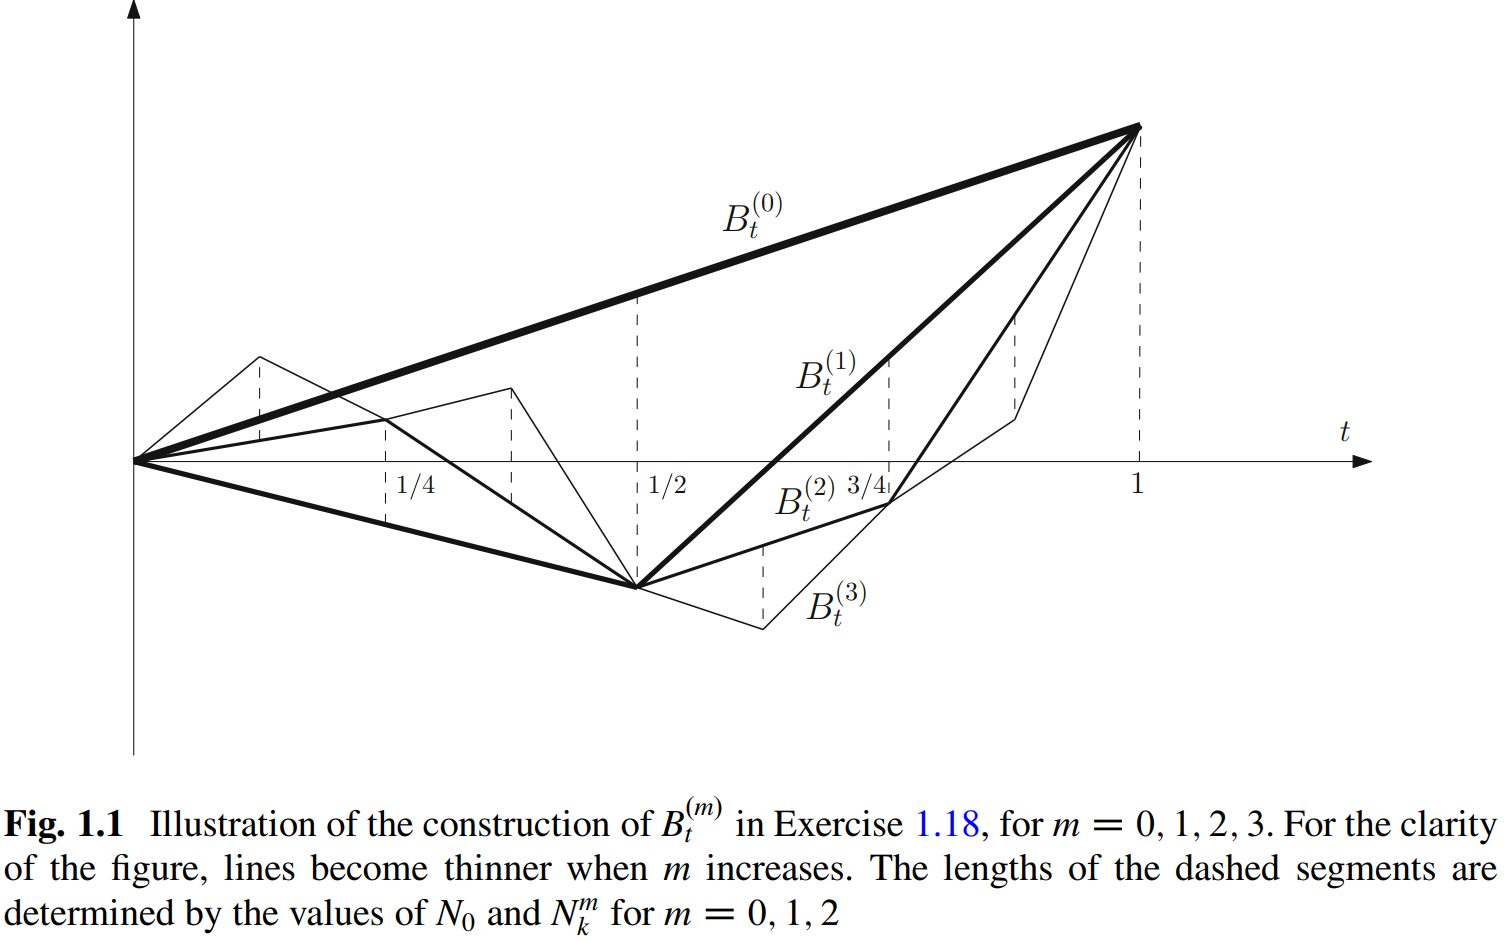
\includegraphics[width=0.8\textwidth]{ex_1_18_image.png}
    \end{center}
}

\begin{prob}
    Conclude that we can, for every $t \in [0,1]$, select a random variable $B'_t$ which is a.s. equal to $B_t$, in such a way that the mapping $t \mapsto B'_t(\omega)$ is continuous for every $\omega \in \Omega$.
\end{prob}

A uniformly convergent sequence of continuous functions converges to a continuous function. Thus, it is already almost surely true that $B_t(\omega)$ is continuous, and we can set $B' = B$ in those cases. In the (measure $0$) event that it is not, simply define $B'_t(\omega) = 0$. This is a.s. equal to $B_t$, and now the mapping $t \mapsto B_t(\omega)$ is continuous for every $\omega \in \Omega$.

\end{document}